\documentclass[a4paper,12pt]{article}
  \usepackage{amssymb}
  \usepackage{graphicx}
  \usepackage{indentfirst}
  \title{U-Net: Convolutional Networks for Biomedical Image Segmentation}
  \author{Olaf Ronneberger \emph{et al.}}
  \date{2015}

\begin{document}
\maketitle

\section{Contribution}

In this paper, we modify and extend the so-called "fully convolutional network" such that it works with very few training images and yields more precise segmentations.

One important modification in our architecture is that in the upsampling part we have also a large number of feature channels, which allow the network to propagate context information to higher resolution layers.

\section{Network Architecture}

The network architecture is illustrated in Figure 1. It consists of a contracting path (left side) and an expansive path (right side).

\begin{figure}[ht]
	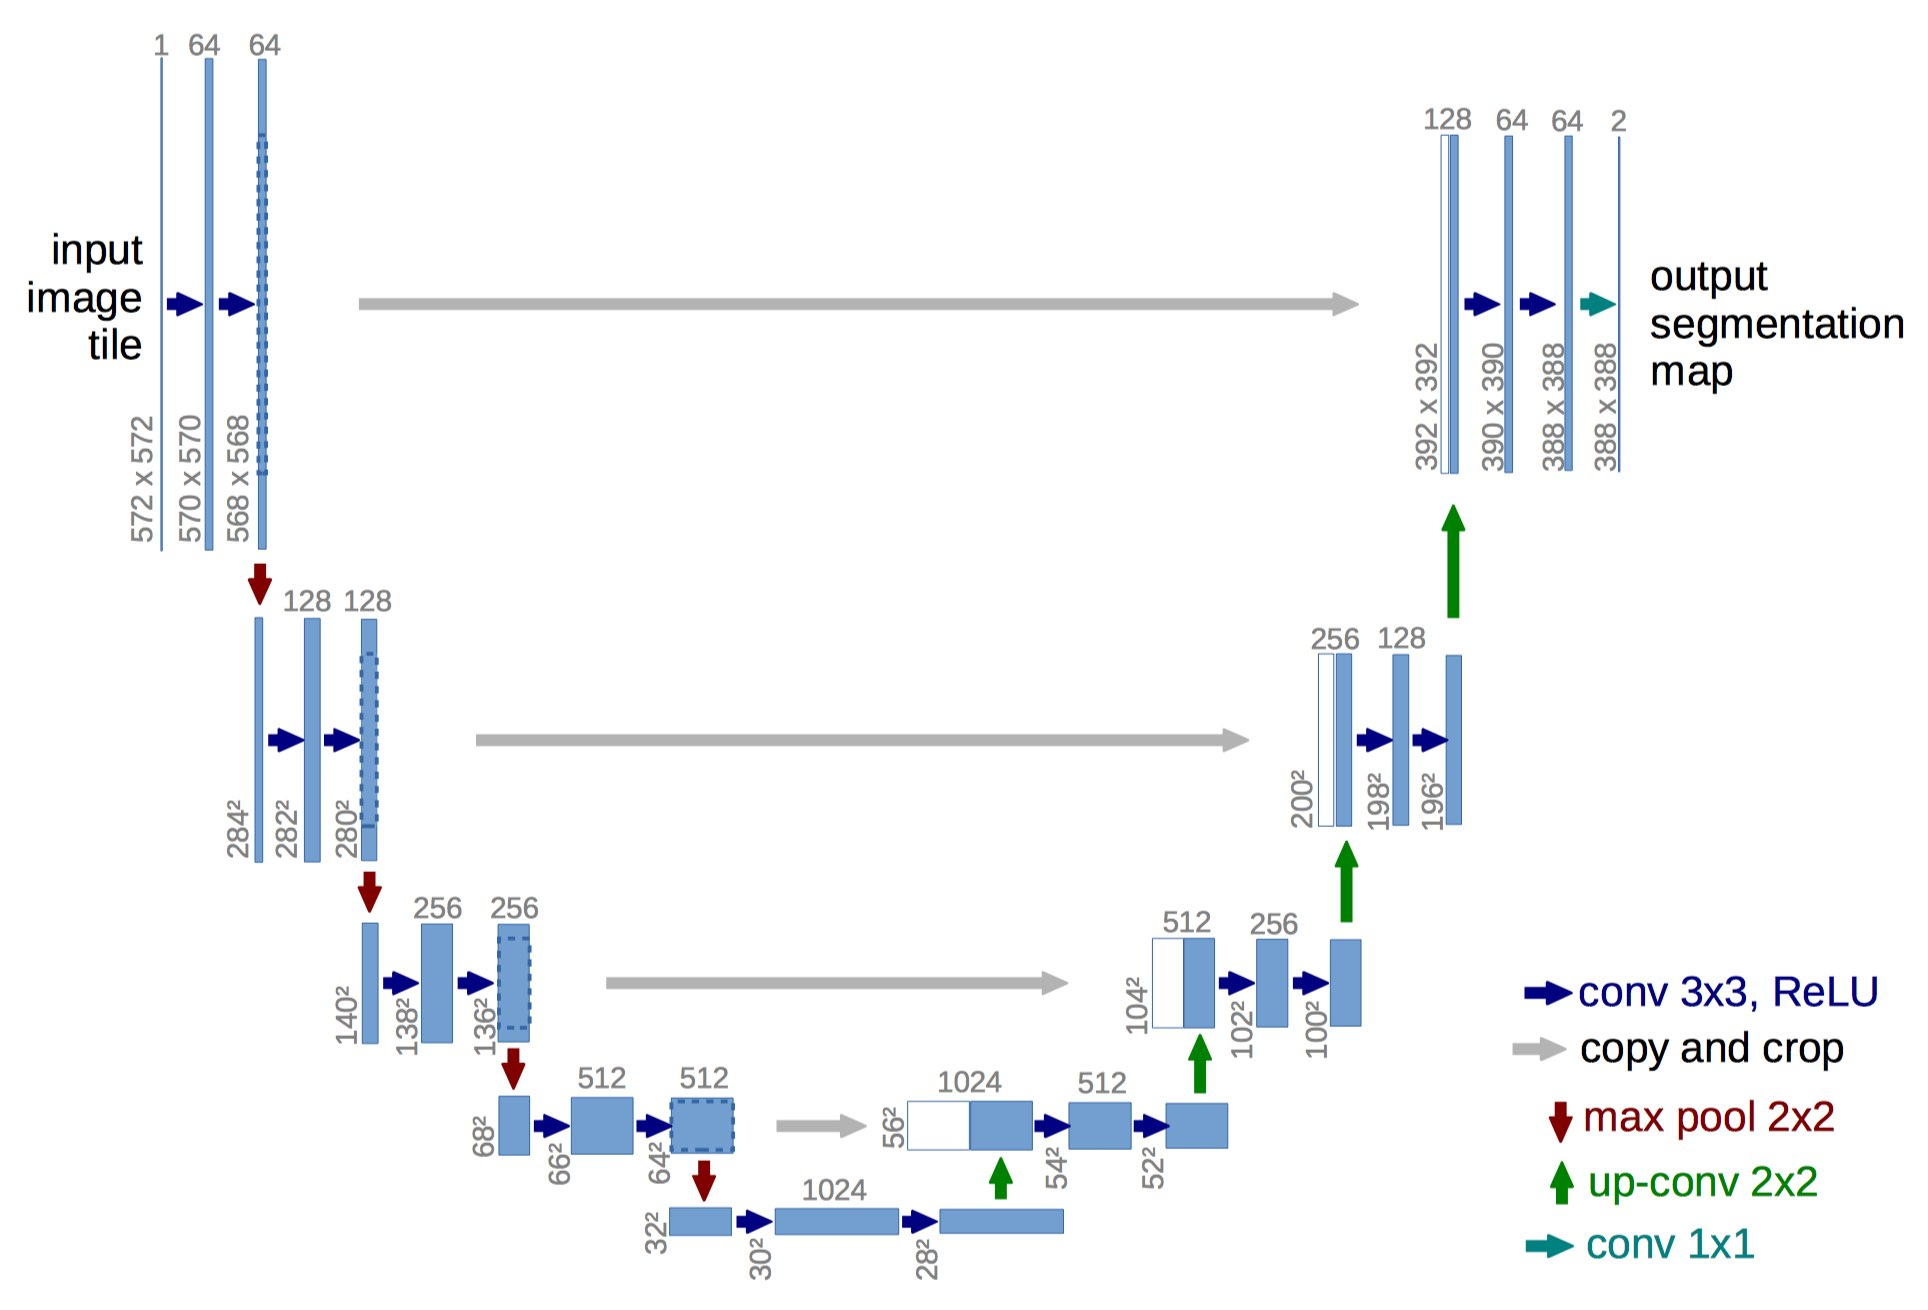
\includegraphics[width=\columnwidth]{img/u-net.jpg}
	\caption{U-net architecture (example for $32 \times 32$ pixels in the lowest resolution). Each blue box corresponds to a multi-channel feature map. The number of channels is denoted on top of the box. The x-y-size is provided at the lower left edge of the box. White boxes represent copied feature maps. The arrows denote the different operations.}
\end{figure}

To allow a seamless tiling of the output segmentation map (see Figure 2), it is important to select the input tile size such that all $2 \times 2$ max-pooling operations are applied to a layer with an even x- and y-size.

\begin{figure}[ht]
	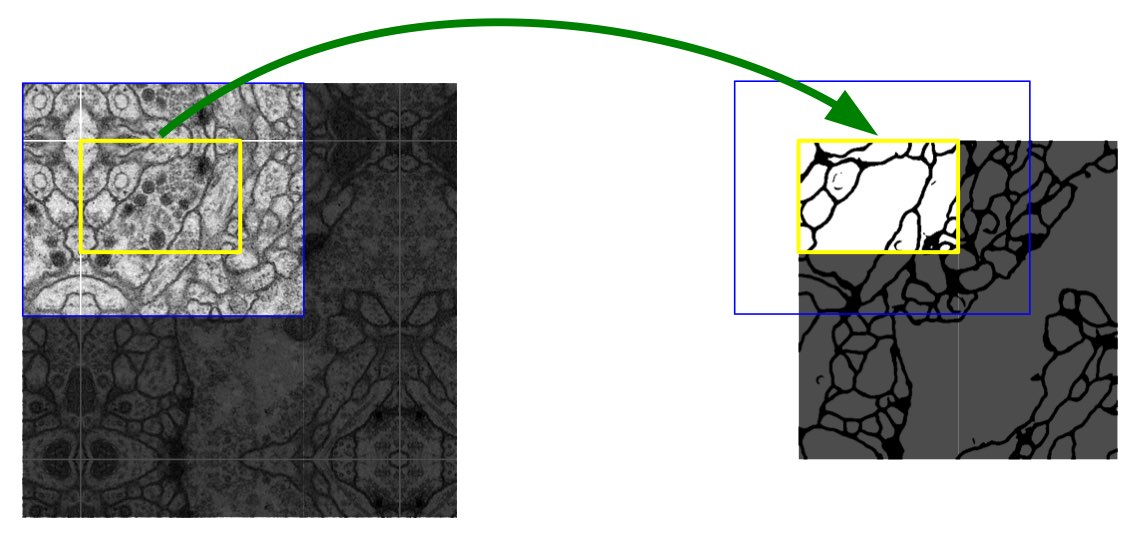
\includegraphics[width=\columnwidth]{img/overlap-tile.jpg}
	\caption{Overlap-tile strategy for seamless segmentation of arbitrary large images (here segmentation of neuronal structures in EM stacks). Prediction of the segmentation in the yellow area, requires image data within the blue area as input. Missing input data is extrapolated by mirroring.}
\end{figure}

\section{Training}

To minimize the overhead and make maximum use of the GPU memory, we favor large input tiles over a large batch size and hence reduce the batch to a single image. Accordingly we use a high momentum (0.99) such that a large number of the previously seen training samples determine the update in the current optimization step.

\subsection{Energy Function}

The energy function is computed by a pixel-wise soft-max over the final feature map combined with the cross entropy loss function. The soft-max is defined as \[p_k(\mathbf{x}) = \frac{\exp(a_k(\mathbf{x}))}{\sum_{k'=1}^K{\exp(a_{k'}(\mathbf{x}))}}\] where $a_k(\mathbf{x})$ denotes the activation in feature channel $k$ at the pixel position $x \in \Omega$ with $\Omega \subset \mathbb{Z}$. $K$ is the number of classes and $p_k(\mathbf{x})$ is the approximated maximum-function.

The cross entropy then penalizes at each position the deviation of $p_{l(\mathbf{x})}(\mathbf{x})$ from $1$ using

\begin{equation}
E = \sum_{\mathbf{x} \in \Omega}w(\mathbf{x})\log(p_{l(\mathbf{x})}(\mathbf{x}))
\end{equation}

where $l : \Omega \to \{1,\ldots,K\}$ is the true label of each pixel and $w : \Omega \to \mathbb{R}$ is a weight map introduced to give some pixels more importance in the training, which is computed as

\begin{equation}
w(\mathbf{x}) = w_c(\mathbf{x}) + w_0 \cdot \exp\left(-\frac{(d_1(\mathbf{x}) + d_2(\mathbf{x}))^2}{2\sigma^2}\right)
\end{equation}

where $w_c : \Omega \to \mathbb{R}$ is the weight map to balance the class frequencies, $d_1 : \Omega \to \mathbb{R}$ denotes the distance to the border of the nearest cell and $d_2 : \Omega \to \mathbb{R}$ the distance to the border of the second nearest cell. In our experiments we set $w_0 = 10$ and $\sigma \approx 5$ pixels.

\subsection{Weights Initialization}

For a network with our architecture (alternating convolution and ReLU layers), weights can be initialized from a Gaussian distribution with a standard deviation of $\sqrt{2 / N}$, where $N$ denotes the number of incoming nodes of one neuron.

\subsection{Data Augmentation}

As for our tasks there is very little training data available, we use excessive data augmentation by applying elastic deformations to the available training images. This is particularly important in biomedical segmentation, since deformation used to be the most common variation in tissue and realistic deformations can be simulated efficiently.

We generate smooth deformations using random displacement vectors on a coarse $3 \times 3$ grid. The displacements are sampled from a Gaussian distribution with $10$ pixels standard deviation. Per-pixel displacements are then computed using bicubic interpolation.

\end{document}
